% main_bsiMC_ufu.tex v1.1, Thiago Pirola Ribeiro
% adaptado do modelo PPGCO - main_ppgco_ufu.tex v1.0, Lásaro Camargos e Denise Guliato
% Criacao: 2019-03-08 - v1.0
% ------------------------------------------------------------------------
% Atualizações.
% 2022-10-18 - v1.1 - Thiago Pirola Ribeiro
% 2025-05-22 - V1.2 - Diego Nunes Molinos
% 2025-09-05 - V1.2 - Diego Nunes Molinos
%                    - Inclusão do texto IA-Generativa
%                    - Retirada dos tópicos opcionais
%                    - Inclusão do texto Observação em vermelho
% 2025-03-12 - V1.3 - Diego Nunes Molinos
%          - Atualização do termo grau para Título de Bacharel;
%          - Inclusão da seção de Abstract;
% ------------------------------------------------------------------------
\documentclass{bsimc}
%Não altere o comando seguinte. O título de seu trabalho será especificado mais adiante.
\title{Observatório da Jornada do Paciente Oncológico}

% ---
% Pacotes fundamentais
% ---
% cmap omitido: fontenc já é carregado por bsimc.cls (abnTeX2)
\usepackage{lmodern}				% Usa a fonte Latin Modern
% Substituições para combinações bold+smallcaps inexistentes em Latin Modern
\AtBeginDocument{%
	\DeclareFontShape{T1}{lmr}{bx}{sc}{<->ssub*lmr/bx/n}{}%
	\DeclareFontShape{T1}{lmss}{bx}{sc}{<->ssub*lmss/bx/n}{}%
}
\usepackage{makeidx}            	% Cria o indice
\usepackage{lastpage}			% Usado pela Ficha catalográfica
\usepackage{indentfirst}			% Indenta o primeiro parágrafo de cada seção.
\usepackage{nomencl} 			% Lista de simbolos
\usepackage{graphicx}			% Inclusão de gráficos
\usepackage{float}
% ---

% ---
% Pacotes adicionais
% ---
\usepackage[printonlyused]{acronym}
\usepackage[table]{xcolor}
% ---

% ---
% Insira aqui os pacotes utilizados por você
% ---
\usepackage{tabularx}
\usepackage{booktabs}
\usepackage{url}
\usepackage{listings}
\usepackage{textcomp}

% Evita warning do hyperref com \uppercase nos títulos de apêndice/anexo (abnTeX2)
\pdfstringdefDisableCommands{%
	\def\uppercase#1{#1}%
}

% ---
% Informações de dados para CAPA e FOLHA DE ROSTO
% ---
%
% Título:
%	1. Título em português
%	2. Título em inglês
\titulo{Observatório da Jornada do Paciente Oncológico: plataforma web pública para exploração de dados de tempo de espera no tratamento oncológico no SUS}{Observatory of the Oncology Patient Journey: a public web platform for exploring cancer treatment waiting-time data in Brazil's SUS}

% Colocar aqui ate 5 palavras-chave do trabalho
\keyword{visualização de dados}
\keyword{saúde pública}
\keyword{React}
\keyword{Registro Hospitalar de Câncer}
\keyword{transparência}

%
% Autor:
%	1. Nome completo do autor
%	2. Formato de nome para bibliografia
\autor{Gustavo Montenegro Felici}{Felici, G. M.}
% Cidade
\local{Uberlândia - MG}
%
% Ano de defesa
\date{2026}
% Área de concentração da pesquisa
\areaconcentracao{Sistemas de Informação}
% Nome do orientador
\orientador{Fernanda Santos}
% Nome do coorientador, se houver
%\coorientador{Nome completo do coorientador}
% -


% informações do PDF
\hypersetup{
	pdftitle={\imprimirtitulo},
	pdfauthor={\imprimirautor},
	pdfsubject={\imprimirpreambulo},
%	pdfkeywords=\@resumokw,
	pdfproducer={LaTeX with abnTeX2}, 	% producer of the document
	colorlinks=true,       		% false: boxed links; true: colored links
	linkcolor=black,          	% color of internal links
	citecolor=black,        		% color of links to bibliography
	filecolor=magenta,      		% color of file links
	urlcolor=black,
	bookmarksdepth=4
}

% ---
% compila o indice
% ---
\makeindex
% ---

% ---
% Compila a lista de abreviaturas e siglas
% ---
\makenomenclature
% ---

% ----
% Início do documento
% ----

\begin{document}

	% ----------------------------------------------------------
	% ELEMENTOS PRÉ-TEXTUAIS
	% ----------------------------------------------------------
	\pretextual

	% ---
	% Insere Capa, Folha de rosto, Ficha catalográfica (se inserida)
	% e folha de aprovação (se inserida).
	% ---
	\maketitle

	% ---
	% Dedicatória - obrigatório somente para TCC 2
	% ---
	\imprimirdedicatoria{Dedico este trabalho à minha família e a todas as pessoas que acreditam no papel da informação como instrumento de cuidado e cidadania.}
	% ---

	% ---
	% Agradecimentos - obrigatório somente para TCC 2
	% ---
	\imprimiragradecimentos{
		Agradeço à orientadora Fernanda Santos pelo acompanhamento e pelas orientações ao longo do desenvolvimento deste Relatório Técnico Profissional.
		Agradeço também à Faculdade de Computação da Universidade Federal de Uberlândia e aos docentes do curso de Sistemas de Informação, cuja formação tornou possível a realização deste trabalho.
		Por fim, agradeço à minha família e aos amigos pelo apoio constante durante a jornada acadêmica.
	}
	% ---

	% ---
	% Epígrafe - obrigatório somente para TCC 2
	% ---
	\imprimirepigrafe{
		``Informação acessível é um passo necessário para decisões mais conscientes em saúde pública.''\\
		(Autor)
	}
	% ---

	% ---
	% RESUMO - obrigatório somente para TCC 2
	% ---

	% Resumo em português
	\begin{resumo}{}

		Este Relatório Técnico Profissional apresenta o desenvolvimento do \textit{Observatório da Jornada do Paciente Oncológico}, uma plataforma web pública voltada à exploração de dados oficiais sobre o tempo decorrido entre o diagnóstico de câncer e o início do tratamento no \acs{SUS}. O objetivo geral foi disponibilizar, de forma acessível a gestores, profissionais de saúde, pesquisadores e cidadãos, indicadores derivados do \acs{IRHC} do \acs{INCA}, permitindo a comparação com o prazo normativo de sessenta dias previsto na Lei nº~12.732/2012, e capacitando esses públicos a extrair suas próprias interpretações e conclusões sobre os padrões observados. A solução foi implementada como aplicação de página única (\acs{SPA}) com React e Vite, precedida por um pipeline de pré-processamento em Node.js que transforma o arquivo \acs{CSV} do \acs{RHC} em agregados \acs{JSON} consumidos no navegador. A interface oferece painéis de indicadores, mapa por Unidade da Federação, recortes por variáveis sociodemográficas e clínicas, e filtros de perfil. Os resultados técnicos incluem a disponibilização de uma base agregada com 1.693.381 registros processados (1.258.486 com datas válidas para o cálculo do tempo de espera) e uma interface estática, sem autenticação, adequada à publicação pública. Conclui-se que a plataforma contribui para a transparência e para a análise exploratória dos dados, ampliando o acesso à informação oficial.

	\end{resumo}

    % Abstract (o argumento define as Keywords em inglês)
	\begin{abstract}{Data visualization. Public health. React. Hospital Cancer Registry. Transparency.}

		This Professional Technical Report presents the development of the \textit{Observatory of the Oncology Patient Journey}, a public web platform for exploring official data on the time between cancer diagnosis and treatment initiation in Brazil's Unified Health System (\acs{SUS}). The main goal was to make indicators derived from the Hospital Cancer Registry (\acs{IRHC}/\acs{INCA}) accessible to managers, health professionals, researchers, and citizens, enabling comparison with the sixty-day normative deadline established by Law No.~12.732/2012, and empowering these audiences to draw their own interpretations and conclusions about the observed patterns. The solution was implemented as a single-page application (\acs{SPA}) with React and Vite, preceded by a Node.js preprocessing pipeline that transforms the \acs{RHC} \acs{CSV} file into \acs{JSON} aggregates consumed in the browser. The interface provides indicator panels, a state-level map, sociodemographic and clinical breakdowns, and profile filters. Technical results include an aggregated dataset of 1,693,381 processed records (1,258,486 with valid dates for waiting-time calculation) and a static, authentication-free interface suitable for public release. The platform contributes to transparency and exploratory analysis, expanding access to official information.

	\end{abstract}

	% ---
	% inserir lista de ilustrações
	% ---
	\listailustracoes
	% ---

	% ---
	% inserir lista de tabelas
	% ---
	\listatabelas
	% ---

	% ---
	% inserir lista de abreviaturas e siglas
	% ---
	\listasiglas{abrev/Abreviaturas}
	% ---

   	% IA Generativa
	\begin{IA-Generativa}{}

	De acordo com o Código de Conduta para pessoas autoras de publicações da Sociedade Brasileira de Computação (SBC), Parte II, Art. 2º, inciso III:

        \textit{III – Uso de Inteligência Artificial (IA) Generativa: a utilização de ferramentas e tecnologias de IA Generativa para geração de conteúdos, na escrita e/ou revisão do conteúdo de artigos, deve ser declarada explicitamente no trabalho. A declaração pode ocorrer na Seção de Agradecimentos, na metodologia ou em uma seção definida especificamente para este fim, de acordo com o template adotado, e deve listar as ferramentas e descrever onde foram empregadas, por exemplo, textos, tabelas, gráficos, citações, etc. Essas ferramentas não podem ser listadas como autores de um artigo. O uso de tais ferramentas não exime os autores da responsabilidade sobre todo o seu conteúdo, inclusive no caso de ser identificado plágio.}

       \noindent O manual completo encontra-se disponível em: \url{https://sol.sbc.org.br/index.php/indice/conduta}

       \vspace{1em}
       \noindent Neste trabalho, ferramentas de Inteligência Artificial Generativa (assistente Cursor com modelo Grok) foram utilizadas para apoio na redação e organização textual dos capítulos em \LaTeX{}, na estruturação de seções a partir da análise do código-fonte da aplicação React e na elaboração de entradas bibliográficas preliminares. A revisão técnica, a validação dos dados apresentados e a responsabilidade pelo conteúdo final são do autor.

	\end{IA-Generativa}

	% ---
	% inserir o sumario
	% ---
	\sumario
	% ---

	% ----------------------------------------------------------
	% ELEMENTOS TEXTUAIS
	% ----------------------------------------------------------
	\mainmatter


	% ----------------------------------------------------------
	% Introdução
	% ----------------------------------------------------------
	\chapter[Introdução]{Introdução}
\label{cap:introducao}

Este Relatório Técnico Profissional foi desenvolvido no âmbito do curso de Bacharelado em Sistemas de Informação da Universidade Federal de Uberlândia, com o intuito de aplicar conhecimentos de engenharia de software, visualização de informação e dados públicos à construção de uma solução técnica real: o \textit{Observatório da Jornada do Paciente Oncológico}. Trata-se de uma plataforma web pública destinada a disponibilizar, de forma compreensível, indicadores derivados de registros oficiais sobre o tempo entre o diagnóstico de câncer e o início do tratamento no \acs{SUS}.

\section{Contextualização do trabalho}

No Brasil, a Lei nº~12.732/2012 estabelece que o paciente com neoplasia maligna tem direito a iniciar o tratamento no \acs{SUS} em prazo máximo de sessenta dias a partir do diagnóstico \cite{lei12732}. Paralelamente, o \acs{INCA} mantém o \acs{IRHC} (também referido como \acs{RHC}), base de dados hospitalares que registra informações clínicas e sociodemográficas de~pacientes oncológicos \cite{inca_irhc}.

Embora esses dados existam e sejam de interesse público, sua forma bruta --- tipicamente arquivos volumosos em \acs{CSV}, com campos codificados e necessidade de tratamento estatístico --- dificulta o acesso por gestores, profissionais de saúde, pesquisadores e cidadãos sem formação específica em análise de dados. A ausência de uma interface pública, estável e orientada à exploração dificulta o uso desses registros como instrumento de transparência e de apoio à análise.

Nesse contexto, o presente trabalho propõe uma plataforma de visualização que:
\begin{itemize}
	\item centraliza indicadores pré-agregados a partir do \acs{IRHC};
	\item apresenta o tempo de espera em linguagem acessível, com referência ao prazo legal de sessenta dias como marco normativo de comparação;
	\item oferece recortes geográficos, sociodemográficos e clínicos para que o usuário explore os dados;
	\item capacita o leitor a formular suas próprias interpretações a partir dos indicadores apresentados.
\end{itemize}

A solução foi concebida para publicação pública, podendo ser utilizada tanto por órgãos e gestores interessados em acompanhar indicadores quanto por qualquer cidadão que deseje conhecer o panorama descrito pelos dados oficiais.

\section{Objetivos Profissionais}

\subsection{Objetivo geral}

Desenvolver e documentar uma plataforma web pública que disponibilize a exploração de indicadores de tempo entre diagnóstico e início do tratamento oncológico, com base em dados do \acs{IRHC}/\acs{INCA}, de modo a ampliar o acesso à informação para governo e sociedade e a apoiar análises conduzidas pelos próprios usuários.

\subsection{Objetivos específicos}

\begin{itemize}
	\item Levantar requisitos de transparência e usabilidade para uma interface pública de exploração de dados de saúde.
	\item Definir regras de cálculo do tempo de espera e critérios de exclusão de registros com datas inválidas.
	\item Implementar um pipeline de pré-processamento capaz de transformar o \acs{CSV} do \acs{RHC} em agregados \acs{JSON} adequados ao consumo no navegador.
	\item Construir a interface em React com painéis de indicadores, mapa por Unidade da Federação, recortes por variáveis e filtros de perfil.
	\item Validar funcionalmente a aplicação e documentar limitações metodológicas dos dados e da solução.
\end{itemize}

\section{Contribuições Esperadas}

As principais contribuições deste Relatório Técnico Profissional incluem:

\begin{itemize}
	\item A entrega de um produto técnico funcional --- aplicação web estática --- apto a ser publicado sem necessidade de backend ou autenticação.
	\item A sistematização de um pipeline reproduzível de agregação de dados do \acs{IRHC} para visualização interativa.
	\item A demonstração da aplicabilidade de conhecimentos de Sistemas de Informação (arquitetura front-end, engenharia de dados leve e design de interfaces) a um problema de interesse público.
	\item A disponibilização de um instrumento de análise exploratória que preserva a autonomia interpretativa do usuário.
\end{itemize}

\section{Organização do Relatório}

Este relatório está estruturado em quatro capítulos textuais, além dos elementos pré e pós-textuais. O Capítulo~\ref{cap:fundamentacao} apresenta a fundamentação técnica e o contexto das tecnologias e conceitos utilizados. O Capítulo~\ref{estudo} detalha a metodologia de desenvolvimento, a arquitetura, os módulos implementados, os testes e o cronograma. O Capítulo~\ref{cap:conclusao} reúne considerações finais, limitações e perspectivas futuras.

\section{IA-Generativa}

De acordo com o Código de Conduta para pessoas autoras de publicações da Sociedade Brasileira de Computação (SBC), Parte II, Art. 2º, inciso III, o uso de Inteligência Artificial Generativa deve ser declarado explicitamente no trabalho \cite{sbc_conduta}.

Neste relatório, ferramentas de IA generativa foram empregadas como apoio à redação e à organização do texto em \LaTeX{}, a partir da análise do código-fonte da aplicação. O autor permanece integralmente responsável pelo conteúdo, pela veracidade das informações técnicas e pela revisão final.



	% ----------------------------------------------------------
	% Fundamentação Prática
	% ----------------------------------------------------------
	\chapter[Contexto e Fundamentação Técnica]{Contexto e Fundamentação Técnica}
\label{cap:fundamentacao}

Este capítulo apresenta o ambiente de aplicação do trabalho, as tecnologias adotadas e os conceitos que embasam a solução. O foco é fundamentar as escolhas técnicas que permitiram construir uma plataforma pública de exploração de dados do \acs{IRHC}, com ênfase em transparência e em comunicação de indicadores que favoreça a análise autônoma pelo usuário.

\section{Ambiente de Atuação}

O projeto foi desenvolvido no contexto acadêmico do curso de Sistemas de Informação, com aplicação prática voltada ao domínio da saúde pública e da transparência de dados. Não se trata de um sistema interno de uma organização privada, mas de uma solução pensada para disponibilização pública a gestores, profissionais, pesquisadores e cidadãos.

A demanda prática identificada foi a dificuldade de acesso e interpretação dos registros do \acs{IRHC} em sua forma bruta. O volume de dados --- da ordem de milhões de linhas --- e a necessidade de tratamento (validação de datas, agregações e mapeamento de códigos) tornam o uso direto do arquivo \acs{CSV} pouco viável para o público geral. A plataforma proposta atua, portanto, como camada de apresentação e exploração sobre agregados pré-calculados.

\subsection{Atribuições do aluno}

O aluno foi responsável pelo ciclo completo da solução técnica, incluindo:
\begin{itemize}
	\item definição das regras de cálculo do tempo de espera e dos critérios de exclusão;
	\item implementação do script de pré-processamento em Node.js;
	\item desenvolvimento da interface React (layout, componentes de visualização e filtros);
	\item integração dos arquivos \acs{JSON} estáticos à aplicação;
	\item validação funcional e documentação do trabalho.
\end{itemize}

\section{Marco normativo e fonte de dados}

Segundo \citeonline{lei12732}, a Lei nº~12.732/2012 estabelece o prazo máximo de sessenta dias para o início do tratamento oncológico no \acs{SUS} após o diagnóstico. No Observatório, esse prazo é utilizado como \textbf{referência normativa de comparação} nos indicadores (por exemplo, percentual de casos com tempo superior a sessenta dias), e não como veredito sobre a qualidade do sistema de saúde. A referência completa da lei consta na seção de Referências deste relatório.

A fonte de dados é o \acs{IRHC}/\acs{RHC} disponibilizado pelo \acs{INCA} \cite{inca_irhc}. Os registros hospitalares incluem, entre outros campos, datas de diagnóstico e de início de tratamento, Unidade da Federação de residência, sexo, raça/cor, escolaridade, estadiamento e localização do tumor. A plataforma não altera os microdados originais: ela agrega e apresenta estatísticas derivadas, com exclusão explícita de registros sem datas válidas para o cálculo do intervalo.

\section{Ferramentas e Tecnologias Adotadas}

As tecnologias foram selecionadas com base em maturidade, documentação, adequação a uma aplicação estática pública e curva de aprendizado compatível com o prazo do trabalho. A Tabela~\ref{tab:tecnologias} resume o conjunto adotado; as documentações oficiais de React, Vite, Recharts e D3 embasam as escolhas \cite{react_docs,vite_docs,recharts_docs,d3_docs}.

\begin{table}[H]
\centering
\caption{Tecnologias adotadas no projeto}
\label{tab:tecnologias}
\begin{tabularx}{\textwidth}{|l|l|X|X|}
\hline
\textbf{Tecnologia} & \textbf{Tipo} & \textbf{Finalidade} & \textbf{Justificativa} \\
\hline
React 19 & Biblioteca de \acs{UI} & Interface interativa baseada em componentes & Ecossistema consolidado e adequado a \acs{SPA} \\
\hline
Vite & Empacotador / \textit{dev server} & Desenvolvimento e build estático & Build rápido e publicação sem servidor de aplicação \\
\hline
Node.js & Runtime & Pré-processamento do \acs{CSV} & Streaming de arquivos grandes e geração de \acs{JSON} \\
\hline
Recharts & Biblioteca de gráficos & Séries temporais e distribuições & Integração nativa com React \\
\hline
d3-geo & Cartografia & Projeção e desenho do mapa do Brasil & Controle fino de \acs{SVG} geográfico \\
\hline
Tailwind CSS & Estilização & Tokens e utilitários de layout & Consistência visual e produtividade \\
\hline
\end{tabularx}
\end{table}

\section{Arquitetura baseada em componentes e SPA estática}

O React organiza a interface em componentes reutilizáveis, com estado local e composição hierárquica \cite{react_docs}. A aplicação do Observatório é uma \acs{SPA}: uma única página com navegação por âncoras (\texttt{\#lei}, \texttt{\#mapa}, \texttt{\#desigualdade}, \texttt{\#explore}, entre outras), sem roteador client-side dedicado. Na prática, o usuário carrega um conjunto de arquivos estáticos (HTML, JavaScript, CSS e \acs{JSON}) e interage com a interface sem novas requisições a um servidor de aplicação.

A decisão de publicar a aplicação como site estático (build Vite) elimina a necessidade de backend, autenticação e banco de dados em tempo de execução. Os dados já agregados são servidos como arquivos em \texttt{public/data/} e carregados via \texttt{fetch} no navegador.

Entre os \textbf{benefícios} dessa abordagem no contexto do projeto, destacam-se:
\begin{itemize}
	\item facilidade de \textit{deploy} em qualquer hospedagem de arquivos estáticos (incluindo portais institucionais);
	\item redução da superfície de ataque, por não expor APIs autenticadas nem banco de dados online;
	\item transparência: os artefatos de dados e o código da interface podem ser inspecionados e republicados;
	\item custo operacional baixo, adequado a uma iniciativa de acesso público à informação.
\end{itemize}

Entre as \textbf{limitações}, destacam-se:
\begin{itemize}
	\item necessidade de pré-processamento offline sempre que a base \acs{CSV} for atualizada;
	\item ausência de personalização por usuário logado ou de gravação de preferências no servidor;
	\item escalabilidade de leitura limitada principalmente pela capacidade da rede e do navegador ao carregar os \acs{JSON}, e não por um backend elástico.
\end{itemize}

\section{Visualização de informação}

A visualização de informação busca mapear dados abstratos em representações gráficas que apoiem a percepção de padrões, sem substituir o julgamento do analista \cite{few2009}. No Observatório, foram adotados:

\begin{itemize}
	\item gráficos de barras, linhas e áreas (Recharts) para tendências anuais, distribuição de espera e estadiamento;
	\item mapa coroplético (\acs{SVG} com d3-geo) para comparação entre Unidades da Federação;
	\item tabelas e cartões de \acs{KPI} para médias, medianas e percentuais em relação ao prazo de sessenta dias;
	\item filtros de perfil para exploração combinada de variáveis.
\end{itemize}

A paleta semântica da interface (tons associados a faixas de tempo de espera) auxilia a leitura rápida dos indicadores, mas os rótulos e textos explicativos enfatizam que se trata de comparação com o marco legal, cabendo ao usuário a interpretação dos resultados.

\section{Pré-processamento e agregação offline}

Arquivos \acs{CSV} com mais de um milhão de linhas são inadequados para parsing completo no navegador em dispositivos comuns. Por isso, adotou-se um pipeline offline: um script Node.js lê o \acs{CSV} (codificação latin1), valida datas, calcula o intervalo em dias e grava agregados em \acs{JSON} (\texttt{aggregates.json} e \texttt{profiles.json}).

Essa estratégia separa a camada de preparação de dados da camada de apresentação, alinhando-se a boas práticas de engenharia de software em que transformações custosas ocorrem fora do caminho crítico da interface \cite{sommerville2011}.

\section{Restrições Técnicas e Operacionais}

As restrições a seguir influenciaram diretamente o escopo e as decisões de projeto:

\begin{enumerate}
	\item \textbf{Publicação sem backend:} a solução deveria ser hospedável como site estático, sem servidor de aplicação, autenticação ou banco de dados em produção.
	\item \textbf{Volume do \acs{CSV} do \acs{RHC}:} o arquivo original (centenas de megabytes e mais de um milhão de linhas) inviabiliza o processamento integral no cliente, impondo o pipeline de pré-agregação.
	\item \textbf{Qualidade e completude dos campos:} datas ausentes ou inválidas e categorias ``ignorado'' reduzem a cobertura de alguns indicadores e exigem comunicação explícita na interface.
	\item \textbf{Cobertura hospitalar do registro:} o \acs{IRHC} não representa, necessariamente, toda a população oncológica do país, o que limita generalizações.
	\item \textbf{Prazo acadêmico e recursos:} o desenvolvimento concentrou-se em uma \acs{SPA} com visualizações essenciais, sem API programática nem drill-down municipal na primeira versão.
	\item \textbf{Comunicação dos indicadores:} os textos da interface e do relatório devem capacitar a análise pelo usuário, sem induzir conclusões causais a partir de recortes exploratórios.
\end{enumerate}

\section{Padrões e Boas Práticas Adotadas}

\begin{itemize}
	\item Separação entre pré-processamento (Node.js) e apresentação (React);
	\item Componentização da interface (\texttt{MetricsPanel}, \texttt{BrazilMap}, análise por variáveis, \texttt{SmartFilters});
	\item Estado local com React Hooks, sem biblioteca global de estado, dada a simplicidade do fluxo de dados;
	\item Documentação inline da metodologia na própria interface (seções de metodologia e sobre);
	\item Linguagem orientada à exploração, descrevendo \textit{como} utilizar os recortes e \textit{quais} indicadores são exibidos.
\end{itemize}

\section{Justificativa das Escolhas Tecnológicas}

Os critérios principais foram:

\begin{itemize}
	\item \textbf{Publicação pública:} stack estática reduz barreira de hospedagem para governo ou sociedade civil;
	\item \textbf{Curva de aprendizado e documentação:} React, Vite e Recharts possuem documentação oficial ampla \cite{react_docs,vite_docs,recharts_docs};
	\item \textbf{Desempenho percebido:} agregação offline evita travamentos no navegador;
	\item \textbf{Manutenibilidade:} módulos com responsabilidade clara facilitam evolução futura (por exemplo, novos recortes ou drill-down por município).
\end{itemize}


	% ----------------------------------------------------------
	% Metodologia de Solução Técnica
	% Obrigatório somente para TCC 2
	% ----------------------------------------------------------
	\chapter[Estudo de Caso da Solução Técnica]{Estudo de Caso da Solução Técnica}
\label{estudo}

Este capítulo apresenta a abordagem metodológica e a arquitetura técnica adotadas no desenvolvimento do Observatório da Jornada do Paciente Oncológico. O objetivo é documentar o processo de trabalho, as decisões de implementação e os critérios utilizados para validar a solução como plataforma pública de exploração de dados.

Entende-se como solução técnica desenvolvida, neste contexto, a criação de uma aplicação web de visualização e exploração de indicadores derivados do \acs{IRHC}, incluindo o pipeline de pré-processamento de dados e a interface interativa publicada de forma estática.

\section{Estratégia de Desenvolvimento}

A estratégia utilizada foi iterativo-incremental, com entregas parciais ao longo do ciclo de desenvolvimento. O trabalho combinou práticas de engenharia de software e elementos típicos de projetos de dados:

\begin{itemize}
	\item organização em ciclos curtos de implementação e revisão da interface;
	\item ciclo de vida em camadas: compreensão do problema, preparação dos dados, implementação da \acs{UI}, validação e documentação;
	\item inspiração no \acs{CRISP-DM} para a etapa de dados (compreensão da base, preparação, avaliação da qualidade dos agregados e ``implantação'' via build estático) \cite{crispdm}.
\end{itemize}

A premissa editorial --- disponibilizar informação para que o usuário conduza a própria análise --- foi tratada como requisito transversal: textos, rótulos e seções de metodologia foram revisados para privilegiar a clareza descritiva dos indicadores.

\section{Arquitetura da Solução}

A arquitetura é deliberadamente simples e adequada a uma publicação pública sem servidor de aplicação. A Figura~\ref{fig:arquitetura} ilustra o fluxo completo, da base hospitalar à interface publicada.

\begin{figure}[H]
\centering
% Autor: substituir o quadro abaixo por \includegraphics[width=0.9\textwidth]{figs/arquitetura.png}
\fbox{\parbox{0.92\textwidth}{\centering\vspace{1.2em}
\textit{Inserir diagrama do fluxo:}\\
\texttt{rhc.csv} $\rightarrow$ \texttt{scripts/preprocess.js} $\rightarrow$ \texttt{aggregates.json} / \texttt{profiles.json} $\rightarrow$ React (\texttt{App.jsx} + componentes) $\rightarrow$ build Vite estático.\\[0.4em]
\vspace{1.2em}}}
\caption{Fluxo de dados da solução: do arquivo CSV do RHC ao build estático da aplicação}
\label{fig:arquitetura}
\end{figure}

Os principais elementos são:

\begin{itemize}
	\item \textbf{Camada de preparação de dados:} script Node.js (\texttt{scripts/preprocess.js}) que lê o \acs{CSV} do \acs{RHC}, valida datas, calcula o tempo de espera e gera agregados;
	\item \textbf{Camada de dados estáticos:} arquivos em \texttt{public/data/} (\texttt{aggregates.json}, \texttt{profiles.json}, \texttt{brazil-states.json});
	\item \textbf{Camada de apresentação:} aplicação React 19 empacotada com Vite, carregada no navegador;
	\item \textbf{Ausência de persistência online e de autenticação:} todos os usuários acessam o mesmo conteúdo público.
\end{itemize}

\subsection{Regra de cálculo do tempo de espera}

O indicador central é o número de dias entre a data de diagnóstico (\texttt{DTDIAGNO}) e a data de início do tratamento (\texttt{DATAINITRT}). São considerados válidos apenas intervalos entre 0 e 3.650 dias (dez anos). Datas vazias, sentinelas do tipo \texttt{00/00/0000} ou não interpretáveis no formato dia/mês/ano são excluídas do cálculo.

A partir dos casos válidos, calculam-se média, mediana (via histograma), percentuais acima de 30 e de 60 dias, distribuições por faixas, agregações por Unidade da Federação, ano, escolaridade, raça/cor, sexo, estadiamento e grupo de tumor, além de perfis combinados para o módulo de exploração.

Na base processada para a versão documentada neste relatório, foram obtidos \textbf{1.693.381} registros totais e \textbf{1.258.486} com tempo de espera calculável. A média observada foi de \textbf{135} dias e a mediana de \textbf{68} dias; aproximadamente \textbf{54\%} dos casos válidos apresentaram tempo superior a 60 dias. Esses números são descritivos da base agregada e devem ser interpretados à luz das limitações metodológicas (cobertura hospitalar, exclusões e possíveis fatores de confusão).

\section{Componentes e Módulos Implementados}

A interface é uma página única organizada em seções. Os principais módulos são descritos a seguir. As Figuras~\ref{fig:hero} a~\ref{fig:explore} correspondem a capturas de tela da aplicação em execução; o autor deve substituir os quadros reservados pelas imagens finais em \texttt{figs/}.

\subsection{Shell da aplicação (\texttt{App.jsx})}

Responsável pelo carregamento dos dados (\texttt{loadAndProcess}), pelo estado do perfil de filtros, pela navegação por âncoras e pela composição das seções narrativas (hero, lei, mapa, recortes, explore, metodologia e sobre).

\begin{figure}[H]
\centering
% Autor: 
\includegraphics[width=0.9\textwidth]{figs/hero.png}
\fbox{\parbox{0.92\textwidth}{\centering\vspace{1.5em}
\textit{Inserir captura da tela inicial (hero), com o título da aplicação e os indicadores globais de tempo médio e percentual acima de 60 dias.}\\[0.3em]
\vspace{1.5em}}}
\caption{Tela inicial do Observatório, com indicadores globais de tempo de espera}
\label{fig:hero}
\end{figure}

\subsection{Painel de indicadores (\texttt{MetricsPanel.jsx})}

Apresenta a comparação com o prazo legal de 60 dias, cartões de \acs{KPI}, distribuição do tempo de espera e gráficos de tendência anual, estadiamento e volume de casos (Recharts).

\begin{figure}[H]
\centering
% Autor: \includegraphics[width=0.9\textwidth]{figs/metrics.png}
\fbox{\parbox{0.92\textwidth}{\centering\vspace{1.5em}
\textit{Inserir captura da seção de indicadores (MetricsPanel), com a referência de 60 dias, KPIs e gráficos de tendência.}\\[0.3em]
\vspace{1.5em}}}
\caption{Painel de indicadores em relação ao prazo legal de sessenta dias}
\label{fig:metrics}
\end{figure}

\subsection{Mapa do Brasil (\texttt{BrazilMap.jsx})}

Renderiza um mapa coroplético das Unidades da Federação a partir de GeoJSON, com escala de cores associada ao tempo médio de espera, \textit{tooltip} e ranking lateral. Estados com amostra insuficiente são tratados conforme regras de contagem mínima definidas no pré-processamento.

\begin{figure}[H]
\centering
% Autor: \includegraphics[width=0.9\textwidth]{figs/mapa.png}
\fbox{\parbox{0.92\textwidth}{\centering\vspace{1.5em}
\textit{Inserir captura do mapa coroplético por UF e do ranking lateral de estados.}\\[0.3em]
\vspace{1.5em}}}
\caption{Mapa coroplético do tempo médio de espera por Unidade da Federação}
\label{fig:mapa}
\end{figure}

\subsection{Exploração por variáveis sociodemográficas e clínicas}

O componente de análise por variáveis (arquivo \texttt{InequalityAnalysis.jsx} no código) apresenta tabelas e gráficos que permitem ao usuário \textbf{comparar} indicadores entre categorias de escolaridade, raça/cor e tipo de tumor, além de cruzamentos auxiliares (por exemplo, distribuição de tumores e estadiamento). A interface inclui notas sobre possíveis fatores de confusão e percentuais de informação ignorada, para que a leitura permaneça cautelosa. O texto da aplicação e deste relatório disponibilizam instrumentos para que o leitor conduza a própria análise dos padrões observados.

\begin{figure}[H]
\centering
% Autor: \includegraphics[width=0.9\textwidth]{figs/recortes.png}
\fbox{\parbox{0.92\textwidth}{\centering\vspace{1.5em}
\textit{Inserir captura da seção de recortes por escolaridade, raça/cor e tipo de tumor.}\\[0.3em]
\vspace{1.5em}}}
\caption{Recortes exploratórios por variáveis sociodemográficas e clínicas}
\label{fig:recortes}
\end{figure}

\subsection{Filtros de perfil (\texttt{SmartFilters.jsx})}

Permite combinar sexo, raça/cor, escolaridade e grupo de tumor. Os resultados são obtidos por busca em \texttt{profiles.json} (chave \texttt{sexo|raca|instruc|tumor}), exibindo média, mediana e percentual acima de 60 dias em comparação com a linha de base global. O mesmo componente opera na seção ``Explore'' e em um drawer de filtros no cabeçalho.

\begin{figure}[H]
\centering
% Autor: \includegraphics[width=0.9\textwidth]{figs/explore.png}
\fbox{\parbox{0.92\textwidth}{\centering\vspace{1.5em}
\textit{Inserir captura da seção Explore com filtros de perfil selecionados e indicadores do subconjunto.}\\[0.3em]
\vspace{1.5em}}}
\caption{Exploração por perfil combinado (sexo, raça/cor, escolaridade e tipo de tumor)}
\label{fig:explore}
\end{figure}

\subsection{Utilitário de carga (\texttt{processData.js})}

Centraliza o carregamento de \texttt{aggregates.json} e \texttt{profiles.json}, além de mapas de rótulos (sexo, raça/cor, escolaridade, estadiamento) usados na interface.

\section{Testes Realizados}

Não foi implementada uma suíte automatizada de testes unitários ou de ponta a ponta (por exemplo, Jest ou Cypress). A validação concentrou-se em procedimentos manuais e de engenharia, descritos a seguir.

\subsection{Validação do pré-processamento}

Após cada execução de \texttt{node scripts/preprocess.js}, foram conferidos:
\begin{itemize}
	\item totais de registros (\texttt{totalCases}) e de casos com espera válida (\texttt{totalWithWait});
	\item média e mediana de dias, bem como percentuais acima de 30 e de 60 dias;
	\item coerência das agregações por UF, ano, escolaridade, raça/cor e tumor com as regras de exclusão de datas.
\end{itemize}
Como resultado, a versão documentada neste relatório consolidou 1.693.381 registros processados e 1.258.486 com tempo calculável, sem inconsistências aparentes entre as regras do script e os valores gravados em \texttt{aggregates.json}.

\subsection{Testes funcionais da interface}

Foram exercitados, em navegador desktop:
\begin{itemize}
	\item navegação por âncoras entre as seções da página;
	\item abertura e fechamento do drawer de filtros;
	\item seleção de perfis no \texttt{SmartFilters} e atualização dos indicadores exibidos;
	\item renderização do mapa (incluindo \textit{tooltip}) e dos gráficos Recharts;
	\item leitura das seções de metodologia e sobre, quanto à clareza das limitações.
\end{itemize}
Não foram observados erros de carregamento dos \acs{JSON} nem falhas de renderização nas seções principais durante as rodadas de verificação.

\subsection{Teste de build e empacotamento}

A execução de \texttt{npm run build} (Vite) foi utilizada para verificar a geração do diretório \texttt{dist/} com os assets estáticos. O build concluiu sem erros, confirmando que a aplicação pode ser publicada sem servidor de aplicação.

\subsection{Revisão editorial da interface}

Além dos aspectos funcionais, os textos da \acs{UI} foram revisados para privilegiar formulações que descrevem indicadores e convidam à exploração, em vez de afirmações conclusivas sobre padrões sociais.

\section{Critérios e Métricas de Avaliação}

A avaliação da solução considerou critérios alinhados a uma plataforma pública de exploração de dados, conforme a Tabela~\ref{tab:metricas}.

\begin{table}[H]
\centering
\caption{Critérios e métricas para avaliação da solução}
\label{tab:metricas}
\begin{tabularx}{\textwidth}{|l|X|}
\hline
Critério & Métrica / evidência \\
\hline
Corretude das agregações & Consistência entre regras do preprocess e valores em \texttt{aggregates.json} \\
\hline
Desempenho percebido & Carregamento dos \acs{JSON} e fluidez da \acs{SPA} em navegador desktop \\
\hline
Usabilidade exploratória & Capacidade de obter indicadores globais e por recorte sem treinamento formal \\
\hline
Publicabilidade & Build estático sem dependência de backend ou autenticação \\
\hline
Transparência metodológica & Presença de seções de metodologia/limitações na própria aplicação \\
\hline
Clareza editorial & Textos de apoio orientados à exploração e à autonomia interpretativa do usuário \\
\hline
\end{tabularx}
\end{table}

\section{Cronograma de Execução de Atividades}

O cronograma da Tabela~\ref{tab:cronograma} resume a organização temporal das principais fases, em horizonte semestral típico de um Relatório Técnico Profissional.

\begin{table}[H]
\centering
\caption{Cronograma resumido de atividades do projeto}
\label{tab:cronograma}
\scriptsize
\begin{tabularx}{\textwidth}{|l|c|c|c|c|c|c|}
\hline
\textbf{Atividade} & \textbf{Mês 1} & \textbf{Mês 2} & \textbf{Mês 3} & \textbf{Mês 4} & \textbf{Mês 5} & \textbf{Mês 6} \\
\hline
Levantamento do problema e da base IRHC & X & & & & & \\
\hline
Definição de regras e pipeline de dados & X & X & & & & \\
\hline
Implementação da interface React & & X & X & X & & \\
\hline
Mapa, recortes e filtros de perfil & & & X & X & & \\
\hline
Validação funcional e ajustes editoriais & & & & X & X & \\
\hline
Documentação do RTP / TCC & & & & & X & X \\
\hline
\end{tabularx}
\end{table}

Esse cronograma pode ser ajustado conforme prazos institucionais e orientações da banca, mantendo a sequência lógica dados $\rightarrow$ interface $\rightarrow$ validação $\rightarrow$ documentação.


        % ----------------------------------------------------------
	% Projeto, Implementação e Validação da Solução
	% Obrigatório somente para TCC 2
	% ----------------------------------------------------------
	%\include{cap_projeto/projeto}

        % ----------------------------------------------------------
	% Resultados
	% Obrigatório somente para TCC 2
	% ----------------------------------------------------------
	%\chapter[Aprendizados e Perspectivas]{Aprendizados e Perspectivas}
\label{resultados}

Este capítulo apresenta a análise crítica dos resultados obtidos a partir da implementação da solução. São discutidos os dados coletados nos testes, as evidências qualitativas, comparações com abordagens similares e as limitações técnicas observadas ao longo do desenvolvimento.

\section{Resultados Quantitativos e Qualitativos}

Os resultados quantitativos foram obtidos a partir dos testes de desempenho, confiabilidade e usabilidade, conforme descritos anteriormente. A Tabela~\ref{tab:resultados_quantitativos} resume os principais indicadores obtidos:

\begin{table}[H]
\centering
\caption{Indicadores de desempenho da solução}
\label{tab:resultados_quantitativos}
\begin{tabularx}{\textwidth}{|l|X|}
\hline
\textbf{Métrica} & \textbf{Valor Obtido} \\
\hline
Tempo médio de resposta & 180 ms \\
\hline
Taxa de sucesso das requisições & 99,3\% \\
\hline
Cobertura de testes unitários & 85\% \\
\hline
Disponibilidade durante testes & 100\% (ambiente de homologação) \\
\hline
\end{tabularx}
\end{table}

Além disso, foram obtidos feedbacks qualitativos sobre a usabilidade da aplicação por meio de simulações com usuários e análise heurística. Os pontos positivos mais citados foram a simplicidade da interface e a clareza dos relatórios gerados.

\section{Comparações com Soluções Existentes}

A solução proposta foi comparada com abordagens similares disponíveis no mercado ou em sistemas previamente utilizados pela organização. Em relação às soluções existentes, destacam-se os seguintes diferenciais:

\begin{itemize}
  \item Maior nível de automação e integração com sistemas legados;
  \item Interface responsiva e adaptada a múltiplos dispositivos;
  \item Maior cobertura de funcionalidades em um único sistema consolidado;
  \item Facilidade de manutenção e expansão futura.
\end{itemize}

\section{Interpretação dos Dados}

A análise dos dados obtidos indica que a solução atende de forma satisfatória os requisitos funcionais e não funcionais propostos. O tempo de resposta médio ficou abaixo do limite especificado (300 ms), e a taxa de sucesso de requisições demonstra estabilidade do sistema.

A cobertura dos testes também evidencia um bom nível de confiabilidade na lógica implementada. A aceitação positiva durante as simulações de uso reforça a aplicabilidade prática da ferramenta no ambiente-alvo.

\section{Limitações Observadas}

Apesar dos resultados positivos, algumas limitações técnicas e operacionais foram identificadas:

\begin{itemize}
  \item Dependência de conectividade estável com sistemas externos, o que pode impactar o desempenho em ambientes com infraestrutura limitada;
  \item Ausência de testes em ambiente de produção real com carga de usuários simultâneos elevada;
  \item Algumas funcionalidades foram simplificadas para garantir o escopo viável dentro do tempo do projeto;
  \item A interface administrativa ainda requer melhorias em termos de acessibilidade e personalização.
\end{itemize}

Essas limitações não comprometem o uso da solução, mas devem ser consideradas em futuras evoluções ou implantações em larga escala.



	% ---
	% Finaliza a parte no bookmark do PDF, para que se inicie o bookmark na raiz
	% ---
	\bookmarksetup{startatroot}
	% ---

	% ---
	% Conclusão
	% Obrigatório somente para TCC 2
	% ---
	\chapter[Aprendizados e Perspectivas]{Aprendizados e Perspectivas}
\label{cap:conclusao}

Este capítulo apresenta uma reflexão crítica sobre o desenvolvimento do Observatório da Jornada do Paciente Oncológico, articulando os resultados técnicos aos objetivos do Relatório Técnico Profissional, às limitações enfrentadas e às perspectivas de continuidade.

\section{Aprendizado Individual e Coletivo}

O desenvolvimento da solução exigiu a integração de competências típicas de Sistemas de Informação: engenharia de software front-end, tratamento de dados em volume e design de interfaces para comunicação pública. Em especial, destacam-se:

\begin{itemize}
	\item a compreensão de que dados oficiais, por si só, não garantem transparência --- é necessário oferecer meios de exploração compreensíveis;
	\item a prática de separar preparação de dados (pipeline offline em Node.js) e apresentação (React + Vite), decisão decisiva para viabilizar o uso no navegador diante de mais de um milhão de registros;
	\item o domínio de bibliotecas de visualização (Recharts e d3-geo) aplicadas a um problema real de saúde pública;
	\item a atenção à linguagem da interface: disponibilizar recortes sociodemográficos e geográficos de modo a capacitar o usuário a interpretar os indicadores.
\end{itemize}

Do ponto de vista acadêmico, o trabalho reforçou a articulação entre programação, visualização de informação e responsabilidade ética na comunicação de indicadores de saúde. Coletivamente, a experiência evidenciou o valor de documentar limitações metodológicas junto ao próprio produto, e não apenas no relatório.

\section{Desafios}

Entre os principais desafios enfrentados, e as formas de enfrentá-los, destacam-se:

\begin{itemize}
	\item \textbf{Volume e codificação do \acs{CSV}:} o arquivo do \acs{RHC} (latin1, centenas de megabytes) inviabilizou o parsing no cliente. A solução foi o script \texttt{preprocess.js} com leitura em streaming e geração de \acs{JSON} agregados.
	\item \textbf{Qualidade variável dos campos:} datas inválidas e categorias ``ignorado'' reduziram a cobertura de alguns indicadores. Mitigou-se o problema com regras explícitas de exclusão e com a exposição, na interface, de percentuais de informação ignorada.
	\item \textbf{Equilíbrio editorial:} foi necessário revisar textos da \acs{UI} e do relatório para privilegiar a exploração dos dados, sem induzir o leitor a conclusões pré-estabelecidas.
	\item \textbf{Ausência de suíte automatizada:} compensada por validação funcional manual, inspeção dos agregados e verificação do build Vite a cada entrega relevante.
\end{itemize}

Esses obstáculos reforçaram a importância de tratar a qualidade dos dados e a clareza metodológica como parte do produto entregue ao público.

\section{Avaliação Crítica}

Em relação aos objetivos propostos, a solução entrega uma plataforma pública capaz de:

\begin{itemize}
	\item apresentar indicadores globais de tempo entre diagnóstico e início do tratamento;
	\item permitir comparação descritiva com o prazo legal de sessenta dias \cite{lei12732};
	\item oferecer exploração geográfica e por variáveis, bem como filtros de perfil;
	\item operar sem backend, facilitando publicação para governo e sociedade.
\end{itemize}

Pontos fortes incluem a arquitetura estática, o pipeline reproduzível e a presença de seções de metodologia na própria aplicação. Pontos a melhorar, em uma eventual retomada do ciclo, seriam a introdução precoce de testes automatizados sobre as funções de agregação e a geração sistemática de capturas de tela para a documentação. Ainda assim, a arquitetura escolhida mostrou-se adequada ao escopo e ao propósito de transparência.

\section{Articulação com o Curso ou Formação}

O trabalho dialoga diretamente com disciplinas e competências do curso de Sistemas de Informação, tais como desenvolvimento web, modelagem e tratamento de dados (aqui adaptados a agregados), engenharia de software e interação humano-computador. A experiência evidenciou, ainda, a relevância de formação complementar em visualização de dados e em leitura crítica de indicadores de saúde pública --- temas que atravessam a fronteira entre computação e políticas públicas.

Uma lacuna percebida foi a necessidade de maior formalização de testes automatizados e de documentação de \acs{API} de dados, conteúdos que poderiam ser aprofundados em disciplinas de qualidade de software e de integração de sistemas.

\section{Limitações}

Além dos desafios já citados, reconhecem-se limitações estruturais da solução e da base:

\begin{itemize}
	\item a base \acs{IRHC} é hospitalar e não cobre, necessariamente, todos os casos oncológicos do país \cite{inca_irhc};
	\item diferenças entre grupos podem refletir composição de tumores, estadiamento e outros fatores de confusão, e não relações causais --- cabendo ao usuário a interpretação;
	\item a aplicação atual não oferece drill-down municipal nem \acs{API} programática;
	\item dependência de reprocessamento offline sempre que a base \acs{CSV} for atualizada;
	\item a validação concentrou-se em testes manuais, sem cobertura automatizada contínua.
\end{itemize}

\section{Perspectivas Futuras}

Como desdobramentos possíveis da plataforma, sugerem-se:

\begin{itemize}
	\item aprofundamento geográfico (município ou macrorregião), mantendo regras claras de amostra mínima;
	\item exposição de uma \acs{API} ou de arquivos versionados para reuso por gestores e pesquisadores;
	\item empacotamento como \acs{PWA} para uso offline de agregados já baixados;
	\item suíte de testes automatizados no pipeline de dados (unitários nas funções de agregação e regressão dos totais);
	\item painel de metadados da base (versão do \acs{CSV}, data de processamento, dicionário de campos);
	\item estudos colaborativos com especialistas em epidemiologia para enriquecer as notas metodológicas, preservando o caráter exploratório da ferramenta.
\end{itemize}

Em síntese, o Observatório cumpre o papel de tornar dados públicos mais acessíveis à análise por governo e cidadãos, contribuindo para a transparência e para a autonomia interpretativa do usuário.

	% ----------------------------------------------------------
	% ELEMENTOS PÓS-TEXTUAIS
	% ----------------------------------------------------------
	\postextual

	% ----------------------------------------------------------
	% Referências bibliográficas
	% ----------------------------------------------------------
	\bibliography{bib/modelo-referencias}

	% ----------------------------------------------------------
	% Glossário - opcional
	% ----------------------------------------------------------
	%
	%\glossary

	% ----------------------------------------------------------
	% Apêndices  - opcional
	% O apêndice de demonstração do abnTeX2 foi removido para evitar
	% citações indefinidas e reduzir o tempo de compilação.
	% ----------------------------------------------------------
	%\begin{apendicesenv}
	%	\partapendices
	%	%% abtex2-modelo-include-comandos.tex, v-1.4 laurocesar
%% Copyright 2012-2013 by abnTeX2 group at http://abntex2.googlecode.com/ 
% ---
% Este capítulo, utilizado por diferentes exemplos do abnTeX2, ilustra o uso de
% comandos do abnTeX2 e de LaTeX.
% ---
 
% \chapter[Sobre]{Sobre}
% 
% Este documento e seu código-fonte são exemplos de referência de uso da classe
% \textsf{bsimc.cls} e do pacote \textsf{abntex2cite}. O documento 
% exemplifica a elaboração de trabalho acadêmico (tese, dissertação e outros do
% gênero) produzido conforme a \ac{ABNT} \ac{NBR} 14724:2011 \emph{Informação e documentação - Trabalhos acadêmicos - Apresentação}.
% 
% Este modelo é baseado na implementação das normas  para produção de textos estabelecida pela Universidade de São Paulo e 
% mais especificamente pelo Departamento de Engenharia Elétrica da Escola de Engenharia de São Carlos.
% 
% Permissão para a modificação deste modelo foi dada pelo senhor: Athila Quaresma Santos
 
 
\chapter{Ajuda com comandos}\label{cap_ajuda}

\chapterprecishere{Isto é uma sinopse de capítulo. Não estão sendo colocados itens obrigatórios, porém todos os itens constantes aqui, certamente ajudará no desenvolvimento do TCC.}\index{sinopse de capítulo}

\vspace{10pt}
Um site para ser consultado é \url{https://github.com/abntex/abntex2/wiki/Ferramentas} que dá várias dicas de ferramentas para auxiliar no uso do \LaTeX~. 

% ---
\section{Citações}
% ---

Utilize o ambiente \texttt{citacao} para incluir citações diretas com mais de três linhas:

\begin{citacao}
As citações diretas, no texto, com mais de três linhas, devem ser
destacadas com recuo de 4 cm da margem esquerda, com letra menor que a do texto
utilizado e sem as aspas. No caso de documentos datilografados, deve-se
observar apenas o recuo \cite[5.3]{NBR10520:2002}.
\end{citacao}

Citações simples, com até três linhas, devem ser incluídas com aspas. Observe que em \LaTeX~ as aspas iniciais são diferentes das finais: ``Amor é fogo que arde sem se ver''. 

Para utilizar as referências que você buscou, os comandos mais comuns são:

\begin{itemize}
	\item \begin{verbatim}
		\cite{nome da referência} 
		\end{verbatim}
		Usado para que apareça no texto \textbf{(Ribeiro, 2022)}
	\item \begin{verbatim}
		\citeonline{nome da referência} 
		\end{verbatim}
		Usado para que apareça no texto \textbf{Ribeiro (2022)}
\end{itemize}

% ---
\section{Remissões internas}
% ---

Ao nomear a \autoref{tab-nivinv}, apresentamos um exemplo de remissão interna, que também pode ser feita quando indicamos o \autoref{cap_ajuda}\footnote{O número do capítulo indicado é \ref{cap_ajuda}, que se inicia à página \pageref{cap_ajuda}.}
(\nameref{cap_ajuda}, \autopageref{cap_ajuda}), por exemplo.

% ---
\section{Tabelas}
% ---

Apresenta-se um exemplo de tabela a ser confeccionada. Atente-se para as normas de tabela exigidas pela Universidade.

Existem diversos sites para auxiliar na criação de tabelas para \LaTeX~, por exemplo o \url{http://www.tablesgenerator.com}.

\index{tabelas}A \autoref{tab-nivinv} é um exemplo de tabela construída em
\LaTeX.

\begin{table}[htb]
\footnotesize
\caption[Níveis de investigação]{Níveis de investigação.}
\label{tab-nivinv}
\begin{tabular}{p{2.6cm}|p{6.0cm}|p{2.25cm}|p{3.40cm}}
   \hline
   \textbf{Nível de Investigação} & \textbf{Insumos}  & \textbf{Sistemas de Investigação}  & \textbf{Produtos}  \\
   \hline
   Meta-nível & Filosofia\index{filosofia} da Ciência  & Epistemologia & Paradigma  \\
   Nível do objeto & Paradigmas do meta-nível e evidências do nível inferior & Ciência  & Teorias e modelos \\
   Nível inferior & Modelos e métodos do nível do objeto e problemas do nível inferior & Prática & Solução de problemas  \\
   \hline
\end{tabular}
\legend{Fonte: \citeonline{van86}}
\end{table}

% ---
\section{Expressões matemáticas}
% ---

\index{expressões matemáticas}Use o ambiente \texttt{equation} para escrever
expressões matemáticas numeradas:

\begin{equation}
  \forall x \in X, \quad \exists \: y \leq \epsilon
\end{equation}

Escreva expressões matemáticas entre \$ e \$, como em $ \lim_{x \to \infty}
\exp(-x) = 0 $, para que fiquem na mesma linha.

Também é possível usar colchetes para indicar o início de uma expressão
matemática que não é numerada.

\[
\left|\sum_{i=1}^n a_ib_i\right|
\le
\left(\sum_{i=1}^n a_i^2\right)^{1/2}
\left(\sum_{i=1}^n b_i^2\right)^{1/2}
\]

Consulte mais informações sobre expressões matemáticas em
\url{http://code.google.com/p/abntex2/w/edit/Referencias}.

\section{Figuras}

\index{figuras}Figuras podem ser criadas diretamente em \LaTeX,
como o exemplo da \autoref{fig_circulo}.

\begin{figure}[htb]
	\begin{center}
	    \setlength{\unitlength}{5cm}
		\begin{picture}(1,1)
		\put(0,0){\line(0,1){1}}
		\put(0,0){\line(1,0){1}}
		\put(0,0){\line(1,1){1}}
		\put(0,0){\line(1,2){.5}}
		\put(0,0){\line(1,3){.3333}}
		\put(0,0){\line(1,4){.25}}
		\put(0,0){\line(1,5){.2}}
		\put(0,0){\line(1,6){.1667}}
		\put(0,0){\line(2,1){1}}
		\put(0,0){\line(2,3){.6667}}
		\put(0,0){\line(2,5){.4}}
		\put(0,0){\line(3,1){1}}
		\put(0,0){\line(3,2){1}}
		\put(0,0){\line(3,4){.75}}
		\put(0,0){\line(3,5){.6}}
		\put(0,0){\line(4,1){1}}
		\put(0,0){\line(4,3){1}}
		\put(0,0){\line(4,5){.8}}
		\put(0,0){\line(5,1){1}}
		\put(0,0){\line(5,2){1}}
		\put(0,0){\line(5,3){1}}
		\put(0,0){\line(5,4){1}}
		\put(0,0){\line(5,6){.8333}}
		\put(0,0){\line(6,1){1}}
		\put(0,0){\line(6,5){1}}
		\end{picture}
	\end{center}
	\caption{\label{fig_circulo}A delimitação do espaço}
	\legend{Fonte: Autoria Própria}
\end{figure}

Ou então figuras podem ser incorporadas de arquivos externos, como é o caso da
\autoref{fig_grafico}. Se a figura que ser incluída se tratar de um diagrama, um
gráfico ou uma ilustração que você mesmo produza, priorize o uso de imagens
vetoriais no formato PDF. Com isso, o tamanho do arquivo final do trabalho será
menor, e as imagens terão uma apresentação melhor, principalmente quando
impressas, uma vez que imagens vetorias são perfeitamente escaláveis para
qualquer dimensão. Nesse caso, se for utilizar o Microsoft Excel para produzir
gráficos, ou o Microsoft Word para produzir ilustrações, exporte-os como PDF e
os incorpore ao documento conforme o exemplo abaixo. No entanto, para manter a
coerência no uso de software livre (já que você está usando \LaTeX e \abnTeX),
teste a ferramenta \textsf{InkScape}\index{InkScape}
(\url{http://inkscape.org/}). Ela é uma excelente opção de código-livre para
produzir ilustrações vetoriais, similar ao CorelDraw\index{CorelDraw} ou ao Adobe
Illustrator\index{Adobe Illustrator}. De todo modo, caso não seja possível
utilizar arquivos de imagens como PDF, utilize qualquer outro formato, como
JPEG, GIF, BMP, etc. Nesse caso, você pode tentar aprimorar as imagens
incorporadas com o software livre \textsf{Gimp}\index{Gimp}
(\url{http://www.gimp.org/}). Ele é uma alternativa livre ao Adobe
Photoshop\index{Adobe Photoshop}.

\begin{figure}[htb]
	\begin{center}
	    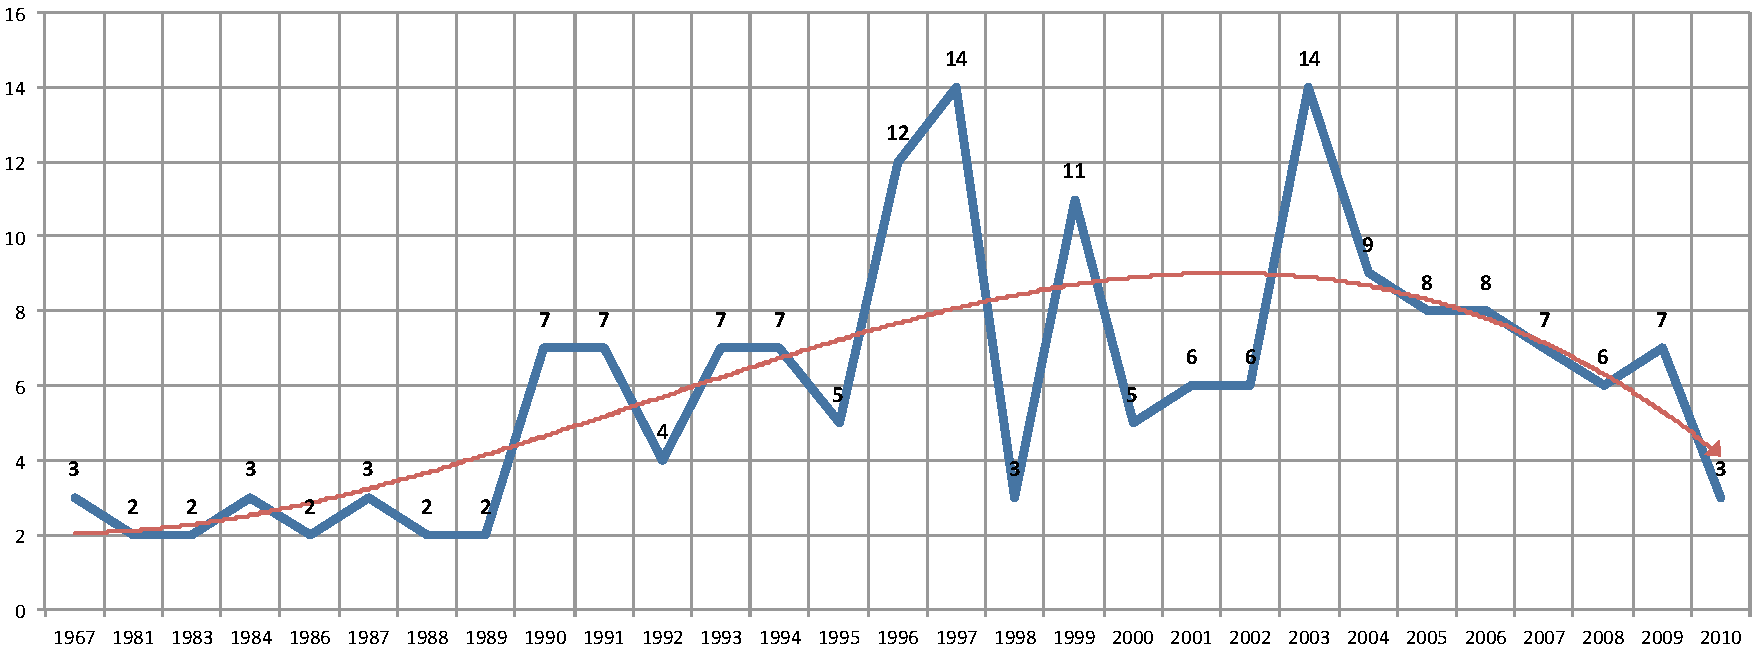
\includegraphics[scale=0.5]{apendices/abntex2-modelo-img-grafico.pdf}
	\end{center}
	\caption{\label{fig_grafico}Gráfico produzido em Excel e salvo como PDF}
	\legend{Fonte: \citeonline[p. 24]{araujo2012}}
\end{figure}

% ---
\section{Enumerações: alíneas e subalíneas}
% ---

\index{alíneas}\index{subalíneas}\index{incisos}Quando for necessário enumerar
os diversos assuntos de uma seção que não possua título, esta deve ser
subdividida em alíneas \cite[4.2]{NBR6024:2012}:

\begin{alineas}

  \item os diversos assuntos que não possuam título próprio, dentro de uma mesma
  seção, devem ser subdivididos em alíneas\footnote{As notas devem ser digitadas ou datilografadas
  dentro das margens, ficando separadas do texto por um espaço simples de entre as
  linhas e por filete de 5 cm, a partir da margem esquerda. Devem ser
  alinhadas, a partir da segunda linha da mesma nota, abaixo da primeira letra
  da primeira palavra, de forma a destacar o expoente, sem espaço entre elas e
  com fonte menor. \citeonline[5.2.1]{NBR14724:2011}}; 
  
  \item o texto que antecede as alíneas termina em dois pontos;
  \item as alíneas devem ser indicadas alfabeticamente, em letra minúscula,
  seguida de parêntese. Utilizam-se letras dobradas, quando esgotadas as
  letras do alfabeto;

  \item as letras indicativas das alíneas devem apresentar recuo em relação à
  margem esquerda;

  \item o texto da alínea deve começar por letra minúscula e terminar em
  ponto-e-vírgula, exceto a última alínea que termina em ponto final;

  \item o texto da alínea deve terminar em dois pontos, se houver subalínea;

  \item a segunda e as seguintes linhas do texto da alínea começa sob a
  primeira letra do texto da própria alínea;
  
  \item subalíneas \cite[4.3]{NBR6024:2012} devem ser conforme as alíneas a
  seguir:

  \begin{alineas}
     \item as subalíneas devem começar por travessão seguido de espaço;

     \item as subalíneas devem apresentar recuo em relação à alínea;

     \item o texto da subalínea deve começar por letra minúscula e terminar em
     ponto-e-vírgula. A última subalínea deve terminar em ponto final, se não
     houver alínea subsequente;

     \item a segunda e as seguintes linhas do texto da subalínea começam sob a
     primeira letra do texto da própria subalínea.
  \end{alineas}
  
  \item no \abnTeX\ estão disponíveis os ambientes \texttt{incisos} e
  \texttt{subalineas}, que em suma são o mesmo que se criar outro nível de
  \texttt{alineas}, como nos exemplos à seguir:
  
  \begin{incisos}
    \item \textit{Um novo inciso em itálico};
  \end{incisos}
  
  \item Alínea em \textbf{negrito}:
  
  \begin{subalineas}
    \item \textit{Uma subalínea em itálico};
    \item \underline{\textit{Uma subalínea em itálico e sublinhado}}; 
  \end{subalineas}
  
  \item Última alínea com \emph{ênfase}.
  
\end{alineas}


% ---
\section{Inclução de outros arquivos}\label{sec-include}
% ---

É uma boa prática dividir o seu documento em diversos arquivos, e não
apenas escrever tudo em um único. Esse recurso foi utilizado neste
documento. Para incluir diferentes arquivos em um arquivo principal,
de modo que cada arquivo incluído fique em uma página diferente, utilize o
comando:

\begin{verbatim}
   \include{documento-a-ser-incluido}      % sem a extensão .tex
\end{verbatim}

Para incluir documentos sem quebra de páginas, utilize:

\begin{verbatim}
   \input{documento-a-ser-incluido}      % sem a extensão .tex
\end{verbatim}

% ---
\section{Compilar o documento \LaTeX}
% ---

Geralmente os editores \LaTeX, como o
TeXlipse\footnote{\url{http://texlipse.sourceforge.net/}}, o
Texmaker\footnote{\url{http://www.xm1math.net/texmaker/}}, entre outros,
compilam os documentos automaticamente, de modo que você não precisa se
preocupar com isso.

No entanto, você pode compilar os documentos \LaTeX usando os seguintes
comandos, que devem ser digitados no \emph{Prompt de Comandos} do Windows ou no
\emph{Terminal} do Mac ou do Linux:

\begin{verbatim}
   pdflatex ARQUIVO_PRINCIPAL.tex
   bibtex ARQUIVO_PRINCIPAL.aux
   makeindex ARQUIVO_PRINCIPAL.idx 
   makeindex ARQUIVO_PRINCIPAL.nlo -s nomencl.ist -o ARQUIVO_PRINCIPAL.nls
   pdflatex ARQUIVO_PRINCIPAL.tex
   pdflatex ARQUIVO_PRINCIPAL.tex
\end{verbatim}

% ---
\section{Divisões do documento: seção}\label{sec-divisoes}
% ---

Esta seção testa o uso de divisões de documentos. Isto é uma seção.

\subsection{Divisões do documento: subseção}

Isto é uma subseção.

\subsubsection{Divisões do documento: subsubseção}

Isto é uma subsubseção.

\subsubsection{Divisões do documento: subsubseção}

Isto é outra subsubseção.

\subsection{Divisões do documento: subseção}\label{sec-exemplo-subsec}

Isto é uma subseção.

\subsubsection{Divisões do documento: subsubseção}

Isto é mais uma subsubseção da \autoref{sec-exemplo-subsec}.

% ---
\section{Este é um exemplo de nome de seção longo. Ele deve estar
alinhado à esquerda e a segunda e demais linhas devem iniciar logo abaixo da
primeira palavra da primeira linha}
% ---

Isso atende à norma \citeonline[seções de 5.2.2 a 5.2.4]{NBR14724:2011} 
 e \citeonline[seções de 3.1 a 3.8]{NBR6024:2012}.


% ---
\section{Consulte o manual da classe \textsf{abntex2}}
% ---

Consulte o manual da classe \textsf{abntex2} \cite{abntex2classe} para uma
referência completa das macros e ambientes disponíveis. Além disso, o manual
possui informações adicionais sobre as normas ABNT observadas pelo \abnTeX.

\section{Referência a Acrônimos}

Exemplos do uso de acrônimo, também conhecidos como siglas: \ac{ABNT} e \ac{TCP}

Ao utilizar uma abreviação, você deve colocá-la no arquivo \texttt{abrev/abreviaturas.tex} e, para utilizar:

\begin{itemize}
	\item \begin{verbatim}
		\ac{nome da referência} 
	\end{verbatim}
	Usado para que apareça no texto \textbf{Protocolo de Controle de Transmissão (TCP)}
	\item \begin{verbatim}
		\acl{nome da referência}  
	\end{verbatim}
	Usado para que apareça no texto \textbf{Protocolo de Controle de Transmissão}
	\item \begin{verbatim}
		\acs{nome da referência}  
	\end{verbatim}
	Usado para que apareça no texto \textbf{TCP}
	\item \begin{verbatim}
		\acsp{nome da referência}  
	\end{verbatim}
	Usado para que apareça no texto \textbf{TCPs}
\end{itemize}

	%\end{apendicesenv}

	% ----------------------------------------------------------
	% Anexos  - opcional
	% ----------------------------------------------------------
	\begin{anexosenv}
		\partanexos
		\chapter{Termo de Ciência e Concordância}
		Documento que atesta a ciência e a concordância da pessoa responsável na empresa em que o discente trabalha ou trabalhou com a publicação deste texto no Repositório Institucional.

		{\color{blue}É necessária a assinatura do documento, com data atualizada, do(a) responsável no Termo de Ciência e Concordância para a publicação do texto do TCC no Repositório Institucional. Baixe o arquivo .docx contido na pasta \texttt{apendices}, preencha e peça a assinatura para incluir o documento aqui. Obs.: este texto deve ser removido na versão final.}

		% Descomente após incluir o PDF assinado:
		% 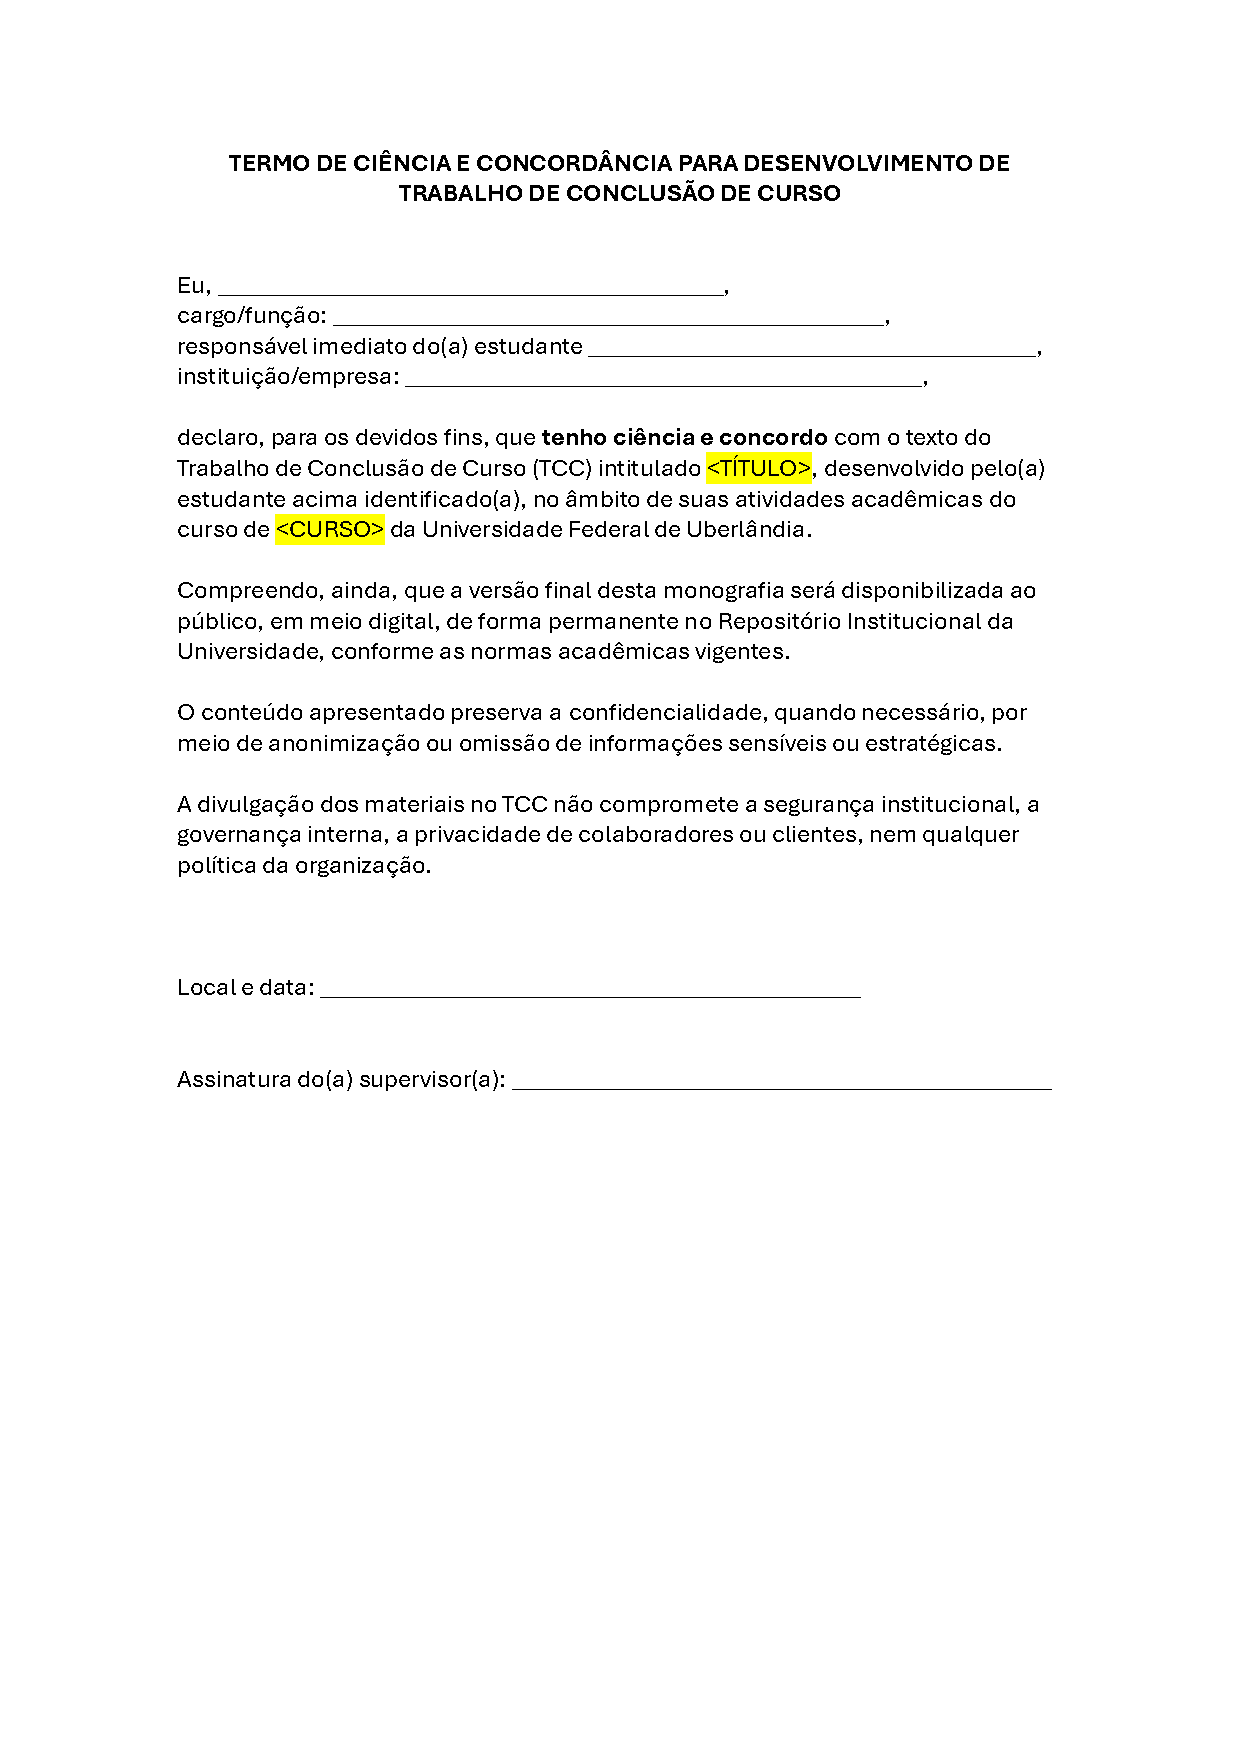
\includepdf{apendices/termo-ciencia-empresa-final.pdf}

	\end{anexosenv}


\end{document}
